\begin{frame}
  \frametitle{Predictions with Decreasing Detector Energy Resolution}
  \begin{figure}
    \centering
    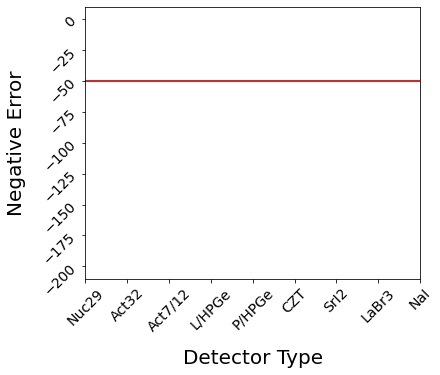
\includegraphics[height=0.7\textheight]{./figures/plot_description.png}
  \end{figure}
\end{frame}

\begin{frame}
  \frametitle{Reactor Type Classification}
  \begin{adjustwidth}{-15pt}{-10pt}
  \begin{figure}
    \centering
    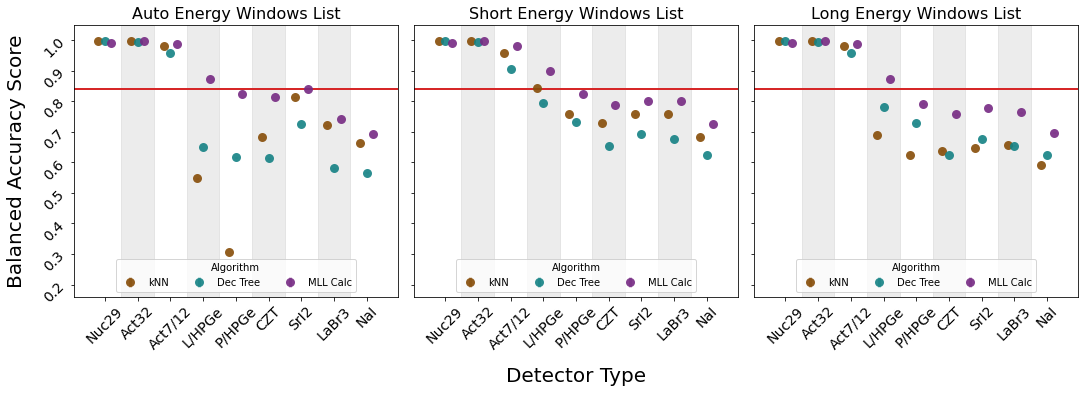
\includegraphics[width=1.1\textwidth]{./figures/detector_preds_wrt_enlist_BalAcc_rxtr.png}
  \end{figure}
  \vspace{12pt} \centering Red baseline: 0.84 balanced accuracy score
  \end{adjustwidth}
\end{frame}

\begin{frame}
  \frametitle{Reactor Type Classification}
  Maybe conf matrices?
\end{frame}

\begin{frame}
  \frametitle{Burnup Regression}
  \begin{adjustwidth}{-15pt}{-10pt}
  \begin{figure}
    \centering
    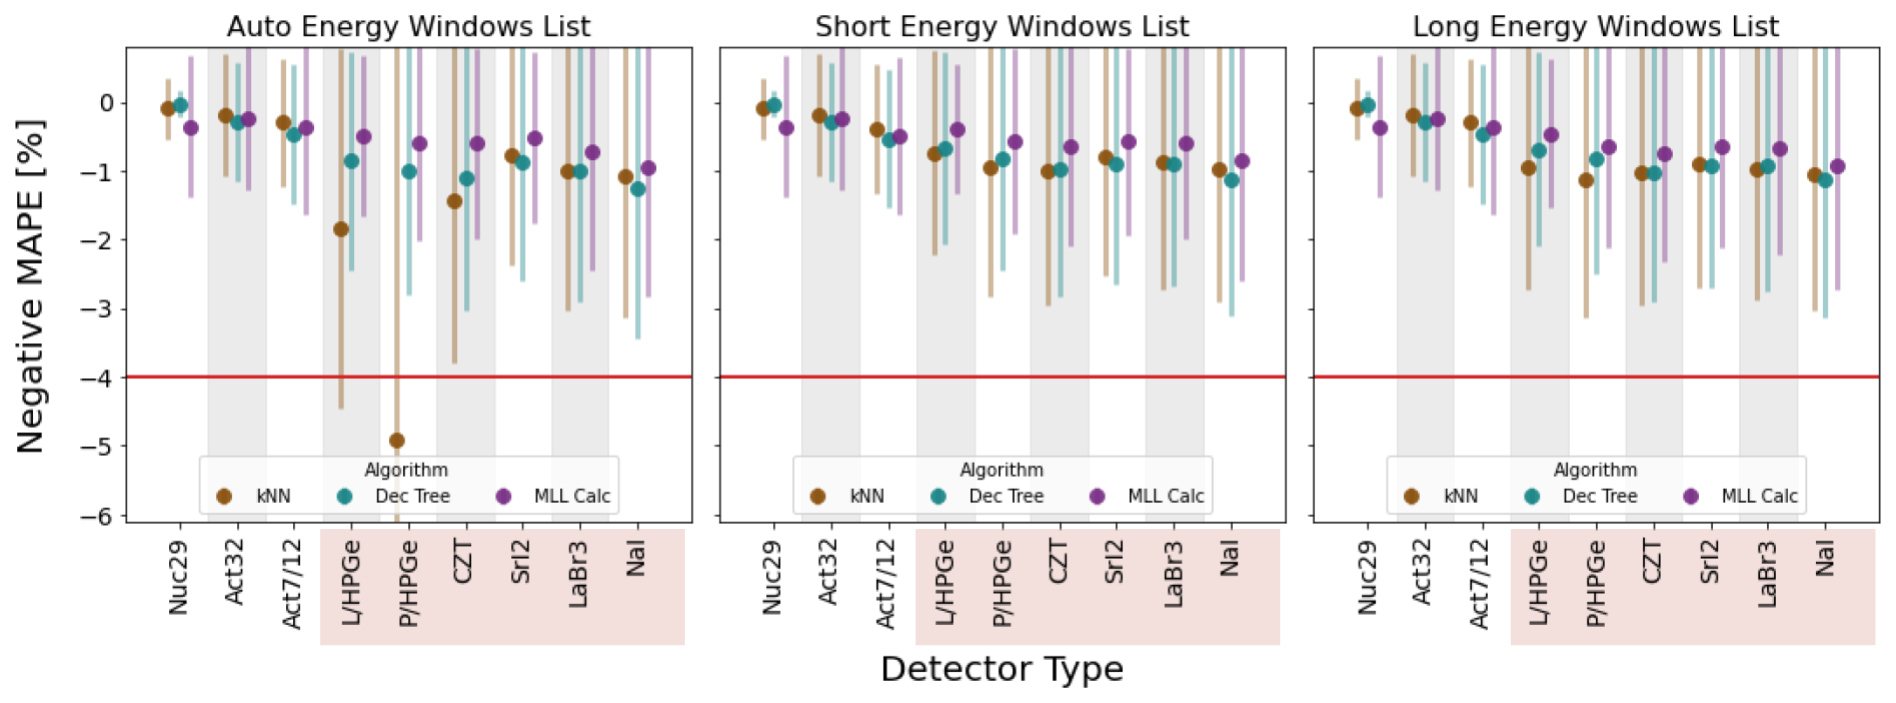
\includegraphics[width=1.1\textwidth]{./figures/detector_preds_wrt_enlist_MAPE_burn.png}
  \end{figure}
  \vspace{12pt} \centering Red baseline: -4\% %$1000\:MWd/MTU$
  \end{adjustwidth}
\end{frame}

\begin{frame}
  \frametitle{${}^{235}\text{U}$ Enrichment Regression}
  \begin{adjustwidth}{-15pt}{-10pt}
  \begin{figure}
    \centering
    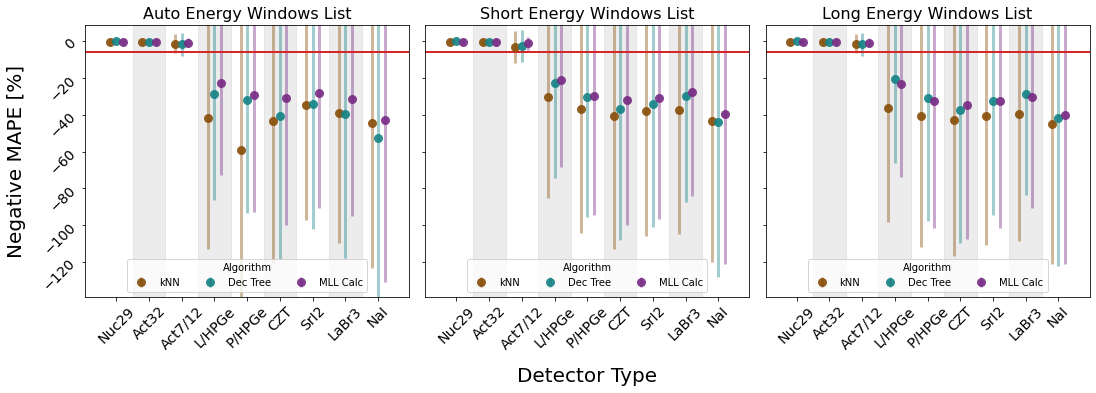
\includegraphics[width=1.1\textwidth]{./figures/detector_preds_wrt_enlist_MAPE_enri.png}
  \end{figure}
  \vspace{12pt} \centering Red baseline: -6\% 
  \end{adjustwidth}
\end{frame}

\begin{frame}
  \frametitle{Time Since Irradiation Regression}
  \begin{adjustwidth}{-15pt}{-10pt}
  \begin{figure}
    \centering
    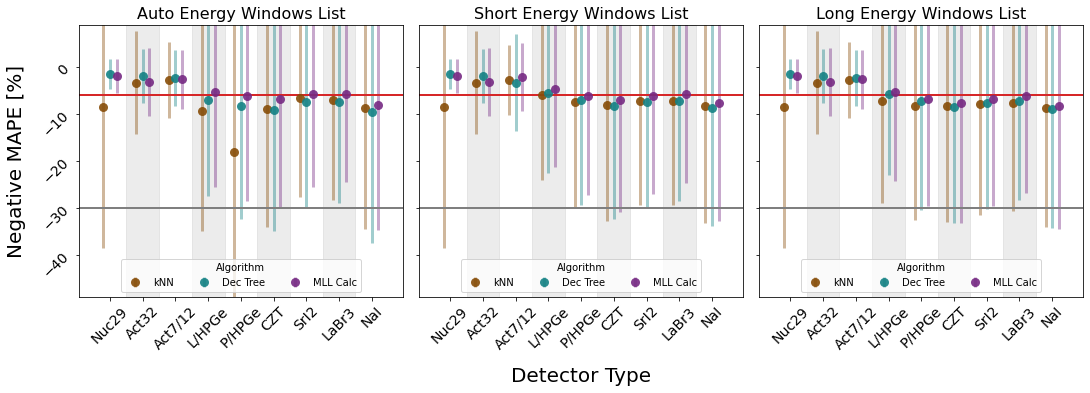
\includegraphics[width=1.1\textwidth]{./figures/detector_preds_wrt_enlist_MAPE_cool.png}
  \end{figure}
  \vspace{12pt} \centering Red baseline: -6\% (Grey line is -30\%) 
  \end{adjustwidth}
\end{frame}


